\chapter{\label{c:speedmeter-control}Concept for the longitudinal control of the \SSM{} experiment}

\newcommand{\RT}{$\textrm{R}_{\textrm{T}}$}

As shown in Chapter\,\ref{c:speedmeter-intro}, the \SSM{} interferometer topology can potentially provide enhanced sensitivity to gravitational waves in the audio-band compared to equivalent \MI{}s. Using as an example the proof-of-concept \SSMEXPT{} in Glasgow, we discuss the issues surrounding the control of this type of interferometer and quantify the challenges using numerical simulations. We present a solution involving the extraction of multiple error signals that can be optimally blended to produce corrective signals to be applied to the test mass actuators. Furthermore we show that this control scheme can be implemented without reducing significantly the quantum non-demolition character of this type of interferometer.

\section{Introduction}
The presence of arm cavities within the \SSMEXPT{} gives rise to challenges not previously encountered in the control of gravitational wave detectors and other experiments involving Michelson or Sagnac interferometers, and this aspect will be addressed in this chapter. In Section\,\ref{sec:ssm-control} we describe in more detail the \SSMEXPT{}, its sensors and actuators and its control requirements. We then describe in Section\,\ref{sec:velocity-control} a control strategy for the \SSM{}'s differential degree of freedom based on that of Michelson designs, and demonstrate the challenges this approach introduces. In Section\,\ref{sec:mixed-control} we present an alternative strategy which achieves adequate control of the interferometer to reach its design sensitivity over extended periods, including a comprehensive noise budget, and derive an optimal filter to combine the two error signals. The parameters used for the control studies are listed in Section\,\ref{sec:control-parameters} and a summary is provided in Section\,\ref{sec:summary}.

\section{\label{sec:ssm-control}Control of the proof-of-concept experiment}

\subsection{\label{sec:ssm-dofs}Degrees of freedom}
Like those of a \FPMI{}, the arm cavities of the \SSM{} must be held resonant in order to maintain the light power required for the design sensitivity, and so these cavities represent a degree of freedom that must be controlled with active feedback. Meanwhile, the error signal is insensitive to the motion of the inter-cavity mode matching mirror, \MNINE{}, since this is situated at half the total round trip distance and is sensed by the counter-propagating modes at almost the same time. Other mirrors are potentially significant: the beam splitter \MSIX{} and steering mirror \MSEVEN{}, as shown in Figure\,\ref{fig:ssm-layout}. As these mirrors are situated near the start of one and the end of the other modes' round trips, a velocity dependent signal is created at the balanced homodyne detector (\gls{BHD}, see Section\,\ref{sec:bhd-intro}). We neglect all other auxiliary optics. To assess the importance of these optics to the interferometer's sensitivity to differential arm cavity length \LMINUS{}, transfer functions from individual mirrors to the \gls{BHD} port were calculated using Optickle (see Appendix\,\ref{sec:optickle-sim}). The results in Figure\,\ref{fig:ssm-mirror-tfs} show that the cavity mirrors are the most important positions to control, with the arm cavity finesse enhancing the sensitivity of the \gls{BHD} to the arm cavity mirrors such that they dominate the signals from \MSIX{} and \MSEVEN{}. \MNINE{}, as expected, is very weakly coupled to the \gls{BHD} port. These results have been confirmed both with Finesse and analytically \cite{Glaefke2015}.

\begin{figure}
  \centering
  \includegraphics[width=\columnwidth]{graphics/generated/from-python/50-mirror-tfs.pdf}
  \caption[Transfer functions from important mirrors/combinations of mirrors in the \SSMEXPT{} to the balanced homodyne detector]{\label{fig:ssm-mirror-tfs}Transfer functions from important mirrors or combinations of mirrors in the \SSMEXPT{} to the balanced homodyne detector. The \LMINUS{} degree of freedom has the strongest response by design. The main beam splitter, \MSIX{}, and the steering mirror for cavity A, \MSEVEN{}, have response approximately one one-hundredth that of \LMINUS{}. Other mirrors, such as \MNINE{}, have significantly lower coupling.}
\end{figure}

While the motion of \MNINE{} can be ruled out as a degree of freedom, being a factor of \SI{e9}{} lower than that of \LMINUS{} below the cavity pole frequency, the effect of \MSIX{} and \MSEVEN{} is less clear cut. To assess the impact the motion from these mirrors has on \LMINUS{} sensitivity, a calculation of the effect of seismic noise from \MSEVEN{} to the \gls{BHD} can be made. \MSIX{} need not be considered separately here for three reasons: the transfer function is almost identical to that of \MSEVEN{} and so we need only calculate one, the beam splitter optic will be heavier than that of \MSEVEN{} and so will couple less seismic noise, and the suspension design\textemdash a work in progress at the time of writing\textemdash is intended to have better isolation than that of \MSEVEN{}'s auxiliary suspension.

Measurements of the seismic motion present upon the ground outside the vacuum system can be propagated through a model of the passive seismic isolation within the vacuum system to obtain the effective seismic motion of the tables upon which the suspensions sit. The seismic motion of \MSEVEN{} can then be calculated by multiplying this spectrum with the transfer function of the auxiliary suspension from the table to the test mass, taken from a state-space model. This seismic noise can be projected into an effective differential arm cavity motion displacement spectral density by multiplying it by the ratio of the transfer functions of \MSEVEN{} and \LMINUS{} to the \gls{BHD} port\footnote{This is the same as multiplying the motion of \MSEVEN{} by its transfer function to the \gls{BHD} port to yield a signal in \SI{}{\watt\per\sqrthz}, and dividing by the transfer function from \LMINUS{} to the \gls{BHD} to yield an effective motion in terms of \LMINUS{}.}, taken from Figure\,\ref{fig:ssm-mirror-tfs}. This can be compared with the requirement for sensitivity of the \gls{BHD} to \LMINUS{}. Figure\,\ref{fig:m7-seismic-noise} shows that \MSEVEN{} will not introduce significant noise above \SI{100}{\hertz}, and from this result we can also conclude that \MSIX{}'s seismic motion will not present a problem.

\begin{figure}
  \centering
  \includegraphics[width=\columnwidth]{graphics/generated/from-python/50-m7-seismic-noise.pdf}
  \caption[Effective \LMINUS{} seismic noise contribution from \MSEVEN{}]{\label{fig:m7-seismic-noise}Effective \LMINUS{} seismic noise contribution from \MSEVEN{}. This is calculated by first propagating a seismic noise spectral density for the laboratory near the vacuum system through damping and suspension models to obtain the motion of the \MSEVEN{} test mass. With this figure, the response at the \gls{BHD} can be calculated from the transfer function shown in Figure\,\ref{fig:ssm-mirror-tfs}, and this in turn can be expressed in units of differential arm cavity motion by dividing it by the response of \LMINUS{} to the \gls{BHD} port. The requirement is given only for frequencies above \SI{100}{\hertz} where the measurement of reduced radiation pressure noise will be made, and this figure shows that seismic motion of \MSEVEN{} will not represent a significant problem to the sensitivity of the experiment in the desired band. This conclusion applies also to the main beam splitter, \MSIX{}, where it is expected that its higher mass will reduce the effect of seismic noise on \LMINUS{} even further.}
\end{figure}

From the results in Figures \ref{fig:ssm-mirror-tfs} and \ref{fig:m7-seismic-noise} it can be concluded that there is only one significant degree of freedom to control in the interferometer in order to meet the sensitivity requirement above \SI{100}{\hertz}, where the measurement of reduced radiation pressure noise will be made. It should, however, be noted that the desired \gls{BHD} homodyne angle depends on the relative path lengths of \MELEVEN{} to \MSIXTEEN{} and \MSIX{} to \MSIXTEEN{}. This length will be controlled by an auxiliary loop not considered part of the longitudinal control strategy, and will be the subject of future work.

\subsection{Sideband frequency}
The eventual choice of sideband frequency, used to control cavity lengths using techniques such as Pound-Drever-Hall (\gls{PDH}, see Section\,\ref{sec:pdh}), will depend on a number of factors both physical and technical. For the purpose of control simulations, however, the only requirement is that the sideband frequency is not resonant within the arm cavities, in order to act as a discriminant to allow for the control of the arm cavity lengths. In practice, this means the frequency offset from the carrier must be greater than the cavity's \gls{FWHM} (see Section\,\ref{sec:cavity-fom}). For control simulations the sideband frequency was chosen to be \SI{15}{\mega\hertz}.

\subsection{\label{sec:simple-control}Control considerations}
Figure\,\ref{fig:simplified-speedmeter-layout-velocity} shows a simplified optical layout of the \SSMEXPT{} with the addition of a basic control loop. The main beam splitter (\MSIX{}) splits the input field towards the two triangular arm cavities where they form counter-propagating modes. One mode from each arm cavity is coupled into the other via the inter-cavity mirror \MNINE{}, and the other modes recombine at the main beam splitter. Here, and for the rest of this chapter, we will consider only the cavity mirrors, the beam splitter and \MNINE{}, defined as shown in Figure\,\ref{fig:simplified-speedmeter-layout-velocity}.

\begin{figure}
  \centering
  \includegraphics[width=0.6\columnwidth]{graphics/generated/from-svg/50-simplified-speedmeter-layout-velocity.pdf}
  \caption[Simplified layout of the \SSMEXPT{} including a basic velocity feedback loop]{\label{fig:simplified-speedmeter-layout-velocity}Simplified \SSM{} layout including extraction of the BHD signal sensitive to the arm cavity differential mode, \LMINUS{}, and the sensing and feedback paths. Light from the input optics (not shown) is incident upon the main beam splitter, \MSIX{}. The triangular arm cavities are shown in the shaded \checkme{grey} area, and mirror \MNINE{} couples light between them. The shaded \checkme{green} area shows the BHD extracting the signal from the main beam splitter's output port (see Section\,\ref{sec:bhd}). The sensing and feedback signal paths are described in detail in Section\,\ref{sec:sensors-and-actuators}.}
\end{figure}

As shown in Section\,\ref{sec:ssm-dofs}, the differential arm cavity length \LMINUS{} is an independent degree of freedom and so frequency-dependent changes lead to frequency-dependent signals at the \gls{BHD}. Motion of an arm cavity mirror imparts signal sidebands upon the counter-propagating modes; these modes have different optical path lengths to the beam splitter and so the signal at the output port contains the superposition of signals representing the mirror's displacement from different points in time, which is analogous to velocity. At \gls{DC} the two modes at the output port contain the same displacement information and the velocity signal is therefore zero\footnote{For a more complete description of the \SSM{}'s behaviour, see, for example, Section\,IIb of \cite{Chen2003}.}.

The error signal (\emph{readout}) representing \LMINUS{} is sensed at the main beam splitter's output port by means of the \gls{BHD} (see Section\,\ref{sec:bhd}) \cite{Steinlechner2015}, as shown in the shaded \checkme{green} area in Figure\,\ref{fig:simplified-speedmeter-layout-velocity}. The frequency dependence of the phase quadrature signal at the \gls{BHD} $s_{\textrm{BHD}}$ is given by the following relationship, ignoring the effect of losses\footnote{A comprehensive treatment of the effect of loss is given in ref.\,\cite{Danilishin2015}.}:
\begin{equation}
  \label{eq:asymdarmbhdresponse}
  s_{\textrm{BHD}} \left( \Omega \right) \propto \frac{\Omega}{ \left(\Omega^2 + \gamma_{\textrm{arm}}^2 \right)} L_{\left(-\right)},
\end{equation}
for angular frequency $\Omega$ and with arm cavity half-bandwidth $\gamma_{\textrm{arm}}$ defined to be:
\begin{equation}
  \gamma_{\textrm{arm}} = \frac{c_{0} T_{\textrm{ITM}}}{4 L_{\textrm{RT}}},
\end{equation}
for speed of light $c_{0}$, arm cavity input test mass (\gls{ITM}) power transmissivity $T_{\textrm{ITM}}$ and arm cavity round-trip length $L_{\textrm{RT}}$.
   
Other terms in the response function dependent upon mirror mass, laser power and mechanical modes are not frequency dependent. Note that for $\Omega \ll \gamma_{\textrm{arm}}$ the response is proportional to frequency, vanishing towards \gls{DC}, as described above and shown in Figure\,\ref{fig:bhd-response}.

\begin{figure}
  \centering
  \includegraphics[width=\columnwidth]{graphics/generated/from-python/50-bhd-response.pdf}
  \caption[The frequency response of the differential arm cavity degree of freedom to the balanced homodyne readout]{\label{fig:bhd-response}The frequency response of \LMINUS{} to the \gls{BHD}, simulated numerically with Optickle. As the \gls{BHD} is sensitive to the arm cavity mirrors' velocity, the signal is proportional to frequency below the cavity pole, and thus zero at \gls{DC}.}
\end{figure}

In order to maintain peak \gls{BHD} sensitivity to \LMINUS{} and therefore gravitational waves, the positions of the cavity mirrors are controlled using \emph{linear inverting feedback}, where an error signal is extracted and applied through a control law to cavity mirror actuators. In the \SSMEXPT{}, voice coils and plate-capacitor electrostatic drives (\glspl{ESD}, see Chapter\,\ref{c:esd-concept}) are used to actuate on the positions of the end test masses (\glspl{ETM}) within each cavity. This feedback maintains the interferometer close to its operating point within the bandwidth of the controller.
   
% For phase noise calculation, see p56 of Lisa Barsotti's thesis
% Or p53 of Rana's thesis
% Or Advanced Virgo design study

\subsection{\label{sec:ssm-required-control}Required precision of the controller}

In order to achieve the required stability, the relative position of the cavity mirrors must be held close to the top of the interference fringe formed by the resonant light, known as the \emph{dark fringe} condition. The noise present within the interferometer, however, produces an unintended \emph{dark-fringe offset} at the output port. The dark fringe condition is strictly only met when there is no interferometer noise, though the slope of the fringe near the minimum is shallow within about 1\% of the fringe's full width at half maximum (\gls{FWHM}, see Section\,\ref{sec:cavity-fom}). A thorough analysis of the required control precision has been derived for the case of a \DRFPMI{} with \gls{DC} readout \cite{Vajente2011} but to the author's knowledge this has not been repeated for a \SSM{} with \gls{BHD} readout. As most technical noise sources in the \SSM{} have similar output port couplings to that of a \MI{}, the requirement is expected to be similar. Assuming that the frequency fluctuations $\Delta f$ fall within \SI{1}{\percent} of the arm cavity \gls{FWHM}, we can derive a requirement to ensure that technical noise sources do not couple strongly to the gravitational wave channel.

Using the parameters listed in Table\,\ref{tab:parameters} with the relation linking laser carrier frequency fluctuations $\Delta f$ and cavity length fluctuations $\Delta L_{\left(-\right)}$,
\begin{equation}
  \frac{\Delta L_{\left(-\right)}}{L_{\textrm{RT}}} = \frac{\Delta f}{f_{0}},
\end{equation}
with $f_{0}$ representing the carrier frequency, the requirement for the \SSMEXPT{} is that the root-mean-square (\gls{RMS}) displacement of the mirrors due to noise must be less than \SI{3.5e-13}{\meter}.

As shown in ref. \cite{Danilishin2015}, asymmetries in the main beam splitter introduce common arm cavity mode coupling at the output port, which leads to further unintended dark fringe offset, and so the real requirement is likely to be more stringent. The controller should therefore have a reasonable factor of safety in terms of the gain it is able to apply to the system to hold it at the operating point.

\subsection{\label{sec:bhd}Balanced homodyne detection}
     
The \gls{BHD} at the \SSMEXPT{}'s output port consists of two high quantum-efficiency photodiodes sensing the reflected and transmitted fields from the \gls{BHD}'s beam splitter, \MSIXTEEN{}. A local oscillator field is incident upon the \gls{BHD}'s beam splitter to provide gain for the velocity information encoded within the light from the main beam splitter, \MSIX{}, itself incident at the other input port of the \gls{BHD}'s beam splitter. The difference current is converted to a voltage by an op-amp with transimpedance resistor \RT{} before being sent to the data acquisition system (\gls{DAQ}).

An example circuit for the balanced homodyne detector is shown in Figure\,\ref{fig:bhd-electronics}. The op-amp introduces its own noise to the output, though a well-chosen op-amp will possess noise significantly lower than the signal representing \LMINUS{} in the intended measurement band. In order for an op-amp to contribute less than \SI{1}{\percent} of the uncorrelated noise in the measurement, its noise must be at least a factor of \SI{10}{} below the dominating noise source in the measurement band\footnote{As the uncorrelated noise sources are added in quadrature, a noise source a factor $\frac{1}{10}$ that of another will contribute approximately $\left(\frac{1}{10}\right)^2 = 1\%$ to the overall noise.}.

\begin{figure}
  \centering
  \includegraphics[width=0.5\columnwidth]{graphics/generated/from-tikz/50-bhd-electronics.pdf}
  \caption[Electronic schematic for the balanced homodyne readout]{\label{fig:bhd-electronics}Simplified electronic schematic for the BHD readout within the \SSMEXPT{}. The difference current from two matched, high quantum efficiency photodiodes is amplified via a transimpedance op-amp stage, with this signal representing the differential motion of the arm cavity mirrors (see Equation\,\ref{eq:asymdarmbhdresponse}).}
\end{figure}

Op-amps used for control in audio-band interferometry typically possess a noise power spectrum inversely proportional to frequency (so-called \emph{flicker noise} \cite[Section\,11.2.3]{Gray2009}) in the low audio band. As the \gls{BHD} error signal is dependent upon the time derivative of the mirror positions, however, there will necessarily be frequencies at which the op-amp noise will dominate the \gls{BHD} error signal. This makes control of slow drifts of the arm cavity mirror positions impossible with the velocity readout, despite the op-amp being well-chosen for a measurement band above \SI{100}{\hertz}. This control problem with relation to the \SSMEXPT{} will be described in more detail in Section\,\ref{sec:velocity-control}.

\subsection{\label{sec:op-amp-noise}Op-amp noise}
To measure the effect of a suitable op-amp's noise at low frequencies, the output from an applicable \gls{BHD} circuit was investigated. The circuit shown in Figure\,\ref{fig:bhd-noise-electronics} was housed within a dark enclosure to minimise photocurrent, with one of the two op-amps within a Texas Instruments\textsuperscript{\textregistered} OPA2227 integrated circuit being used to amplify the noise from the other by a factor of \SI{100}{}. This amplification step is necessary in order to allow the desired op-amp noise to be measured above the noise of the \gls{CDS} data acquisition system's analogue-to-digital converters (\glspl{ADC}) used to record the data. The OPA2227 op-amp is a low-noise precision amplifier designed for audio applications, and is thus suitable for the \gls{BHD} readout in the \SSMEXPT{} depicted in Figure\,\ref{fig:bhd-electronics} given the intended measurement band around a few hundreds of \SI{}{\hertz}. The transimpedance resistor was set to \SI{10}{\kilo\ohm} to balance the first op-amp's contributions to its output from its input current and voltage noise.

\begin{figure}
  \centering
  \includegraphics[width=0.6\columnwidth]{graphics/generated/from-tikz/50-bhd-noise-electronics.pdf}
  \caption[Electronic schematic for the measurement of noise from the balanced homodyne readout]{\label{fig:bhd-noise-electronics}Electronic schematic for the measurement of noise from the BHD readout circuit shown in Figure\,\ref{fig:bhd-electronics}. The output from the transimpedance op-amp is multiplied by a factor of \num{100} by an identical op-amp. The level of multiplication was chosen to allow this noise to exceed the noise of the analogue-to-digital converters within \gls{CDS}.}
\end{figure}

The circuit's output noise was recorded for a period of \SI{16}{} days alongside an open \gls{CDS} input channel used to quantify some of the measurement noise. A time series of the data is shown in Figure\,\ref{fig:op-amp-noise-time-series}, where a drift over the course of the measurement period is apparent. A Fourier transform of the measured op-amp noise time series (Figure\,\ref{fig:op-amp-noise-spectrum}) shows a combination of flicker noise and an additional slope possibly due to resistor current noise below around \SI{1}{\hertz} \cite{Seifert2009}. \gls{ADC} noise dominates above \SI{4}{\hertz}. The ``Model (total)'' spectral density in Figure\,\ref{fig:op-amp-noise-spectrum} shows the contributions to the measurements from the first op-amp $\textrm{N}_{1}$'s current and voltage noise and the Johnson-Nyquist noise of its transimpedance resistor $\textrm{R}_{\textrm{T}}$. This spectral density additionally contains the measured open channel noise summed in quadrature to show the agreement it has with the measurements down to around \SI{1}{\hertz}.

\begin{figure}
  \centering
  \includegraphics[width=\columnwidth]{graphics/generated/from-python/50-op-amp-noise-time-series.pdf}
  \caption[Time series of the noise measured from the balanced homodyne readout electronics]{\label{fig:op-amp-noise-time-series}Time series of the output from the BHD noise measurement circuit shown in Figure\,\ref{fig:bhd-noise-electronics}. The op-amp noise (\checkme{blue}) drifts from \num{0} to a level of approximately \SI{-7.3}{\milli\volt} over the 16 days of measurements. Simultaneously, a CDS channel was measured without an input connected (\checkme{orange}) in order to act as a null stream. The temperature was also measured by a sensor within the same housing as the noise circuit (\checkme{green}), showing a drift of around \SI{0.5}{\celsius}.}
\end{figure}

\begin{figure}
  \centering
  \includegraphics[width=\columnwidth]{graphics/generated/from-python/50-op-amp-noise-spectrum.pdf}
  \caption[Spectral density of the noise measured from the balanced homodyne readout electronics]{\label{fig:op-amp-noise-spectrum}Spectral density of the noise measured from the BHD readout electronics. The op-amp noise spectrum (\checkme{blue}) shows the data in Figure\,\ref{fig:op-amp-noise-time-series} plotted in the frequency domain using Fourier transforms as discussed in Appendix\,\ref{sec:windowing}. The ADC noise spectral density is also given (\checkme{orange}) along with modelled op-amp and resistor noise sources projected into the same measurement point (\checkme{red and purple}, respectively). The most significant contribution to the output is from the first op-amp, as intended; though the noise model, which accounts for the op-amp's input voltage and current noise and the Johnson-Nyquist noise of the resistors, departs from the measurements at lower frequencies.}
\end{figure}

Since the signal measured at the \gls{BHD} in the \SSMEXPT{} represents cavity mirror velocity, it must necessarily drop below the noise at low frequencies where the velocity tends to zero. The op-amp $\textrm{N}_{1}$'s noise drift produces an offset upon the \gls{BHD} error signal which is to be fed back to the cavity mirror actuators, and thus op-amp noise contributes to cavity mirror displacement noise, affecting the experiment's sensitivity.

\subsection{Technical noise}

\subsubsection{\label{sec:adcs-and-dacs}Analogue to digital converters}
The conversion of analogue signals to digital for control and data acquisition by \gls{CDS} hardware involves the use of \glspl{ADC}. Noise in an \gls{ADC} arises from \emph{quantisation error} $\epsilon_{\text{ADC}}$, which is the mismatch between the underlying signal input and the level determined by the \gls{ADC} \cite{Allen1997}. An \gls{ADC}'s job is to take an analogue signal of some voltage and convert it into a corresponding binary word proportional to that input. Some of the fastest \glspl{ADC} work by splitting the input signal into copies and comparing each copy against an increasing threshold voltage\footnote{This is called a \emph{parallel} \gls{ADC}, though there exist many other forms such as \emph{successive approximation}, \emph{voltage-to-frequency}, \emph{integration} and \emph{delta-sigma}. A good overview is given in \cite{Horowitz2015}.}. Initially ignoring additional technical complexity, we can imagine the thresholds of the \gls{ADC} to represent bits of a binary word. The first threshold will check if the input is above or below \SI{1}{\volt}, and output a corresponding high or low signal at that bit location. Subsequent thresholds check for \SI{2}{\volt}, \SI{4}{\volt} and so on. With this simple picture the most obvious flaw is that this system can only determine integer voltage levels, and so $\epsilon_{\text{ADC}} = \SI{0.5}{\volt}$. In reality, however, input signals from interferometer sensors are typically stationary random processes and oscillate between \gls{ADC} thresholds; in effect they are self-dithered. By averaging over successive cycles, the \gls{ADC} can make a better approximation of the underlying signal, reducing the quantisation error to the interval $\epsilon_{\text{ADC}} \in \left( \frac{-\Delta}{2}, \frac{\Delta}{2} \right]$ \cite{Allen1997}, where $\Delta$ is the smallest representable voltage level of an \gls{ADC} of $b$ bits:
\begin{equation}
  \begin{split}
    \Delta &= \frac{V_{\text{max}} - V_{\text{min}}}{2^{b}} \\
           &= \frac{V_{\text{range}}}{2^{b}}.
  \end{split}
\end{equation}

Quantisation noise depends on the noise produced by the components that make up an \gls{ADC}'s threshold sensors, with each contributing noise from its electronics to the output. In the case of the \num{16}-bit \glspl{ADC} in \gls{CDS}, the effective number of bits\footnote{One might decide to purchase an \gls{ADC} based merely upon its number of bits, but this is not a good guide for determining its sensitivity. A 24-bit \gls{ADC} is no better than a noise-free 16-bit \gls{ADC} if the first 8 bits are noise. A more useful figure of merit is the \gls{ENOB}.} (\gls{ENOB}) is $b = 13.9$, corresponding to a noise level of \SI{1.8e-6}{\volt\per\sqrthz} using the relation:
\begin{equation}
  \epsilon_{\text{ADC}} = \frac{V_{\text{range}}}{2^b \sqrt{12 f_{N}}},
\end{equation}
where $f_{N}$ is the Nyquist frequency, which, in the case of \gls{CDS} is \SI{32768}{\hertz}. This noise floor is flat across much of the bandwidth of \gls{CDS} as it is determined by op-amps chosen for low noise in the audio band.

\subsubsection{Digital to analogue converters}
Going from the digital to the analogue domain, the same process happens in reverse with digital to analogue converters (\glspl{DAC}). This time, quantisation noise arises directly from the inability of the \gls{DAC} to faithfully reconstruct the digital signal without adding noise, which is effectively a series of summed voltage thresholds in a similar arrangement to that of an \gls{ADC}. With the \gls{CDS} system, the \glspl{ADC} and \glspl{DAC} are well matched and both possess the same noise floor.

\subsection{\label{sec:sensors-and-actuators}Sensor and actuator dynamic range considerations}

\subsubsection{\label{sec:whitening-dewhitening}Whitening and dewhitening filters}
The signals sensed by the \SSMEXPT{}'s photodetectors contain large components at low frequencies arising from seismic noise, and small components at higher frequencies where the measurement of radiation pressure can be made. The \gls{ADC}'s input range of \SI{\pm10}{\volt} and its noise \SI{1.8e-6}{\volt\per\sqrthz} lead to a dynamic range $\text{D}$ of:
\begin{equation}
  \begin{split}
    \text{D} &= 20 \log_{10} \left( \frac{V_{\text{max}}}{\epsilon_{\text{ADC}}} \right) \\
             &= \SI{134.9}{\deci\bel}.
  \end{split}
\end{equation}
As the sensitivity of the \gls{BHD} is shaped \checkme{approximately inversely to frequency}, signals in the \SI{}{\kilo\hertz} band are typically many orders of magnitude smaller than those of seismic noise at a few \SI{}{\hertz}, meaning that signals at the level of quantum noise are sometimes smaller than the noise of the \glspl{ADC} and \glspl{DAC} and thus nominally undetectable. To avoid this problem, a technique called \emph{whitening} can be utilised. This involves the application of filter to the desired input or output signal in order to increase or decrease certain frequency components of a signal.

The effect of whitening is shown in Figure\,\ref{fig:whitening} for a hypothetical signal and sensor. In the unwhitened case, the signal's dynamic range is greater than that of the sensor, and so the sensor is unable to measure the signal above around \SI{80}{\hertz} with fidelity. At higher frequencies, the signal is below the level of the sensor's noise and as such the sensor cannot distinguish the signal. Most noise sources in gravitational wave interferometry have, however, some inverse frequency dependence at the readout such that the signal content at higher frequencies is smaller than the signal content at lower frequencies. By applying a whitening filter at higher frequencies, the small signal content there can be enhanced to a level at which it can be detected by the sensor above its noise. This effectively reduces the dynamic range of the signal. This is shown in the whitened case. The original signal can be recovered digitally by the application of an inverse whitening filter (``dewhitening'').

The use of whitening can lead to extra noise at higher frequencies, where the continually decaying signal becomes lower than the electronic noise of any real whitening filter arising from the op-amps and resistors. Care must be taken in the design of whitening filters, with components chosen fit for the intended measurement band.

\begin{figure}
  \centering
  \includegraphics[width=\columnwidth]{graphics/generated/from-svg/50-whitening.pdf}
  \caption[The effect of whitening on a signal]{\label{fig:whitening}The effect of whitening on a signal. In the left diagram, the signal's range is greater than that of the sensor. The sensor will in this circumstance be insensitive to signals at frequencies greater than around \SI{80}{\hertz}, assuming that the signal continues to decrease inversely to frequency (as is typical for noise sources in gravitational wave interferometry), instead reading only the noise of the sensor (at $\text{SNR} = 0$). In the right diagram, the signal has had a whitening filter applied to it to increase the signal's magnitude at higher frequencies and thus make it detectable within the dynamic range of the sensor. The underlying, unwhitened signal can be recovered digitally by the application of the inverse whitening filter.}
\end{figure}

The whitening to be applied to the \SSMEXPT{}'s sensor and actuator signals is shown in Figure\,\ref{fig:whitening-tfs}. These filters are sufficient to meet the requirement that the \gls{ADC} and \gls{DAC} noise contribute less than 1\% of the noise power.

\begin{figure}
  \centering
  \includegraphics[width=\columnwidth]{graphics/generated/from-python/50-whitening-filter-tfs.pdf}
  \caption[Input and output whitening filters in the \SSMEXPT{}]{\label{fig:whitening-tfs}Input and output whitening filters in the \SSMEXPT{}. The input whitening will be implemented in the analogue domain whilst the output whitening will be implemented digitally in CDS. The equivalent dewhitening filters will be implemented in the digital and analogue domains, respectively.}
\end{figure}

\subsubsection{Aliasing and imaging}

A consequence of the Nyquist-Shannon sampling theorem is that \gls{AC} signal content can be exactly reconstructed by a sampler if and only if the signal power above the Nyquist frequency is zero \cite{Horowitz2015}. Non-zero signal at frequencies $f > f_{\text{N}}$ will enter the band of the sampler every \checkme{$\frac{f}{f_{\text{N}}}$} cycles and appear on top of the real signal content in that band. To prevent this occurrence, \emph{anti-aliasing} filters can be utilised to aggressively suppress higher frequency content using analogue electronics before the signal is sampled by the \gls{ADC}. Similarly, the output from a \gls{DAC} can be propagated through an \emph{anti-imaging} filter to prevent the \gls{DAC}'s finite sample rate from creating higher frequency copies of in-band signal content.

With \gls{CDS}, the sample frequency is \SI{65536}{\hertz}, and so the Nyquist frequency is \SI{32768}{\hertz}, and the anti-aliasing and anti-imaging filters have cut-off frequency \SI{9}{\kilo\hertz} to ensure that frequency content near the Nyquist frequency is practically zero. The filter is implemented as a \nth{3} order low-pass Butterworth, giving the flattest response in the band up to \SI{9}{\kilo\hertz}. In addition, a notch filter is implemented at the sample frequency to suppress pick-up from the laboratory: ultimately, the sample rate is generated by an oscillator which may produce electromagnetic radiation at nearby frequencies. Figure\,\ref{fig:aa-ai-filter-tfs} shows the (identical) transfer functions of the anti-aliasing and anti-imaging filters implemented in \gls{CDS}. At the Nyquist frequency, the signal is suppressed by approximately \SI{e2}{} and at the sample frequency it is suppressed by \SI{e5}{}.

\begin{figure}
  \centering
  \includegraphics[width=\columnwidth]{graphics/generated/from-python/50-aa-ai-filter-tfs.pdf}
  \caption[Anti-aliasing and anti-imaging filter transfer functions]{\label{fig:aa-ai-filter-tfs}Transfer functions of the anti-aliasing and anti-imaging filters implemented in CDS. The gain at low frequencies is unity to allow signals to pass unperturbed. From \SI{9}{\kilo\hertz}, the filters suppress higher frequency signal content to prevent aliasing or imaging into lower frequencies. At the sample frequency, a notch filter removes all but a factor of \SI{e-5}{} of the signal to prevent pick-up.}
\end{figure}

\subsubsection{\label{sec:sus-gain-hierarchy}Suspension gain hierarchy}

As discussed in Section\,\ref{sec:ssm-actuation} the suspension for each \gls{ETM} will contain two actuator types: voice coils for control of the test mass motion at low frequencies where seismic noise is significant, and an \gls{ESD} for control at high frequencies to correct small but fast perturbations.

The feedback signal generated by the controller within the loop is a signal with frequency components at low and high frequencies, and a set of filters is required to split this feedback between the voice coils and the \glspl{ESD}. This technique is termed \emph{gain hierarchy} and it has been applied for example in the control of \ALIGO{}'s quadruple suspension systems \cite{Shapiro2012}.

Actuators are a potential source of noise in a control loop. Voice coils are susceptible to noise coupling via stray magnetic fields and Barkhausen noise (arising from the discrete magnetic domains in ferromagnets) \cite{Weiss2008}. The \gls{ESD}, however, is anticipated to have excellent noise performance (see Chapter\,\ref{c:esd-concept}), so it would ideally be used for test mass positional corrections across the entire control bandwidth; its maximum voltage supply, and therefore force output, however, is very limited and is nowhere near capable of controlling the test masses due to seismic noise at low frequencies. The \gls{RMS} motion of the uncontrolled \glspl{ETM} is expected to be of the order \SI{e-6}{\meter} due to noise sources such a seismic, thermal, electronic and quantum, while the maximum force output of the \gls{ESD} will be around \SI{1.5}{\micro\newton} (see Chapter\,\ref{c:esd-concept}), corresponding to a displacement of around \SI{690}{\nano\meter} at \SI{1}{\hertz}, or just over half a wavelength. The response of the \gls{ESD} at high frequencies is what would be expected of a force to displacement coupling on a free mass, proportional to $\frac{1}{f^2}$. The voice coils' response at high frequencies, however, contains both a $\frac{1}{f^2}$ slope from force to displacement of the intermediate stage, as well as another $\frac{1}{f^2}$ term from the pendulum stage between the intermediate mass and the test mass, giving an overall filtering effect at high frequencies proportional to $\frac{1}{f^4}$. Given these constraints the effort of the \gls{ESD} is focused at high frequencies where its response is strongest, while the voice coils are utilised at low frequencies where its vastly increased range is available to correct for the larger expected noise disturbances.
% Claim about rms motion of uncontrolled ETM: run /speedmeter/trunk/IfoSimulations/Optickle/projects/noise-budget/plotDiffNoiseBudget.m with large frequency range (e.g. logspace(-2, 5, 1000)), and comment out the line that overrides the rms calculation in the source code
% Maximum ESD force on the ETMs is 1.5 uN, from https://arran.physics.gla.ac.uk/wp/speedmeter/?p=4507. This is multiplied by the force-to-displacement transfer function of the ETM ESD, calculated with Simulink. Use the 1 Hz number, 0.459 m/N.

In order to create the gain hierarchy a series of filters were implemented around a state-space model of the \gls{ETM} suspension. This model includes the response of the actuators from force to displacement for each degree of freedom of the suspension. The use of filters on the input path to each actuator allows us to split the feedback signal into low- and high-frequency corrections, while an overall filter allows common corrections to be applied to both actuators. The control loop built to configure the suspension gain hierarchy is shown in Figure\,\ref{fig:etm-control-loop}.

\begin{figure}
  \centering
  \includegraphics[width=0.7\columnwidth]{graphics/generated/from-svg/50-etm-control-loop.pdf}
  \caption[End test mass suspension control loop block diagram]{\label{fig:etm-control-loop}\gls{ETM} suspension control loop block diagram. The output of the state-space model representing the test mass motion is fed back to the actuators via an ``overall'' servo. This servo can in principle represent the interferometer's response, since the test mass motion from the suspension will be altered by the interferometer before being fed back to the actuators, though in the development of the gain hierarchy the interferometer's response is assumed to be unity. The real effects can be compensated for in the controller (see Section\,\ref{sec:ifo-compensation}).}
\end{figure}

From the control precision requirement presented in Section\,\ref{sec:ssm-required-control} it can be shown that the \gls{RMS} motion as a function of frequency drops below this requirement around \SI{100}{\hertz}, meaning that the interferometer's controller must at least feed back signals up to this frequency. To give the controller some extra headroom to control particularly large noise transients\textemdash expected due to the stationary random noise present within the system\textemdash the unity gain frequency should instead be set at a higher frequency.
% 100 Hz figure is a shaky estimate from https://arran.physics.gla.ac.uk/wp/speedmeter/?p=4455

While the shaping of the hierarchical gain is an iterative process that requires some trial and error, the following paragraphs attempt to explain the methodology behind the features of the \SSMEXPT{}'s implementation for the \glspl{ETM}.

\paragraph{Stable unity gain frequency}
Primarily due to the dynamic range of sensor and actuators, the controller has finite bandwidth and cannot feed back signals at an infinite number of frequencies. The control bandwidth was set to \SI{350}{\hertz} to give a reasonable factor of safety over the \SI{100}{\hertz} requirement. This means the unity gain frequency is \SI{350}{\hertz}. As the \gls{ESD} will be providing most of the feedback at this frequency, we must ensure that its slope is proportional to $\frac{1}{f}$ at \SI{350}{\hertz} to facilitate a stable unity gain crossing (see Section\,\ref{sec:gain-phase-margin}). As the force-to-displacement response is proportional to $\frac{1}{f^2}$ above the pendulum resonance, we want to add an $f$ response to make this $\frac{1}{f}$, and so we use a transitional differentiator between \SI{30}{\hertz} and \SI{1}{\kilo\hertz}.

\paragraph{Stable actuator crossover frequency}
A frequency at which the magnitude of feedback from the voice coils and \gls{ESD} is equal is called a \emph{crossover} frequency. This point has the same requirement as the unity gain frequency, in that the feedback must not be \SI{180}{\degree} out of phase with the input. To facilitate a stable crossover at around \SI{18}{\hertz}\textemdash chosen to prevent the \gls{ESD}'s range from being consumed by low frequency noise\textemdash a transitional differentiator between \SI{2}{\hertz} and \SI{50}{\hertz} was added to the voice coil servo. As the voil coil's high frequency response is proportional to $\frac{1}{f^4}$, this results in a response of $\frac{1}{f^3}$ to compliment the \gls{ESD}'s response of $\frac{1}{f^2}$\textemdash a difference of \SI{90}{\degree}.

\paragraph{Increasing the voice coil feedback at the pendulum resonances}
At \SI{1.8}{\hertz} the final pendulum stage is resonant and so the ground motion is amplified on the test mass. To keep this motion under control an additional boost was provided to the voice coil feedback through a \nth{2} order resonant gain filter with pole and zero at the resonant frequency and a quality factor of around \num{3} to allow for slight changes in the resonant frequency due to temperature drift.

\paragraph{Control of pitch coupling}
At \SI{10.2}{\hertz}, a coupling between pitch and longitudinal modes of the suspension's final stage pendulum leads to a suspension resonance. To prevent this mode from ringing, a \nth{2} order resonant gain filter was applied at \SI{10.2}{\hertz} with a quality factor of \num{4} to allow for manufacturing tolerance. As the voice coil and \gls{ESD} feedback is of similar magnitude at this frequency, this filter was placed within the common feedback path.

\paragraph{Damping of violin modes}
Violin modes (see Section\,\ref{sec:sus-thermal-noise}) are present on the \gls{ETM} suspensions starting at \SI{800}{\hertz}. Although this frequency is well above the control bandwidth, the modes have high enough quality factor and amplitude and are resonant peaks with a \SI{180}{\degree} phase change such that they can potentially lead to positive (unstable) feedback. Instead of damping these modes with resonant gain, we avoid feedback at this frequency by applying a \nth{2} order notch filter. For illustration we've added damping for the first violin mode. If the higher order violin modes become a problem for control we can add additional filters as necessary.

\paragraph{Implementation considerations}
To provide an equal number of poles and zeros in the \gls{ESD} servo, we add an additional transitional differentiator between \SI{0.05}{\hertz} and \SI{5}{\hertz}. This has little effect on the response as the \gls{ESD}'s gain is much smaller than that of the voice coils in this range, but it simplifies the digital implementation of the servo. Ideally, the differentiator's corner frequency would be at \gls{DC}, but this is not possible in a digital implementation.

If low frequency seismic noise must be suppressed further, an extra boost can be applied to the voice coil servo with the inclusion of a transitional integrator between for example \SI{0.01}{\hertz} and \SI{1}{\hertz}, though this has not been considered in the analysis.

The closed-loop transfer functions for the voice coils and \gls{ESD} are shown in Figure\,\ref{fig:suspension-crossover}.

\begin{figure}
  \includegraphics[width=\columnwidth]{graphics/generated/from-python/50-etm-suspension-tfs.pdf}
  \caption[Simulated end test mass suspension actuator closed loop transfer functions]{\label{fig:suspension-crossover}Simulated \SSMEXPT{} ETM suspension actuator closed-loop transfer functions showing the difference in gain between the voice coils and \gls{ESD}. The voice coils provide extensive actuation range but are suppressed at high frequencies by the final stage pendulum. The \gls{ESD} actuates directly upon the test mass and is therefore capable of providing stronger correction than the voice coils at higher frequencies. A \nth{2} order notch filter is present on both actuators at \SI{800}{\hertz} to prevent excitation of the first suspension violin mode.}
\end{figure}

\subsubsection{\label{sec:ifo-compensation}Interferometer compensation}
The suspension gain hierarchy in Section\,\ref{sec:sus-gain-hierarchy} was developed by feeding the test mass motion directly back to the suspension actuators, as shown in Figure\,\ref{fig:etm-control-loop}. In reality, the test mass motion affects the interferometer which changes the signal on the \gls{BHD}, and so the frequency components of the signal are altered. In order for the suspension gain hierarchy to operate as designed, a filter must be placed in the controller to compensate for the interferometer's response. This was implemented in \gls{CDS} as transitional integrators: the first between \SI{0.1}{\hertz} and \SI{2}{\kilo\hertz} and the second between \SI{1}{\hertz} and \SI{100}{\hertz}. While these filters do not reproduce the exact transfer of \LMINUS{} displacement to the \gls{BHD} readout, it approximates it closely enough to allow the suspension gain hierarchy to operate as per its design. During commissioning it will be useful to adjust the shape of this compensation to better fit the real interferometer.

\subsubsection{Photodiode quantum efficiency}
A photodiode's \emph{quantum efficiency} relates to how well it converts incoming photons into electrons. A real photodiode cannot fully convert incoming light power into photocurrent without some loss. Photons not used to produce photoelectrons instead go into heating the substrate, which leads to spontaneous production of electron-hole pairs as current noise.

The number of photons corresponding to a given light power is governed by the wavelength, and a photodiode's efficiency changes with wavelength. To calculate the photocurrent from a photodiode for a given light power at a given wavelength, we use its \emph{responsivity}. For \SI{1064}{\nano\meter} laser light there exists some high quantum efficiency models providing upwards of \SI{0.9}{\ampere\per\watt}, which is the figure we assume for the photodiodes of the \gls{BHD}.

\subsubsection{Loop gain}
With the response of \LMINUS{} to the \gls{BHD} readout calculated by Optickle and implemented in the control loop alongside the suspension feedback and interferometer compensation filters, the strength of the control loop's suppression of displacement noise is determined by the \emph{loop} gain. This is a dimensionless number determined by the response of each component within the loop into its connected components. It can be increased manually through the use of a \gls{DC} gain stage placed anywhere within the loop, or for instance by utilising a photodetector with higher quantum efficiency or by using stronger actuators. It is in practice easiest to place a manual, ``overall'' gain stage within the controller, in this case the \gls{CDS} system where gain is ``free'' within the limit of the voltage range of the \gls{DAC}. An increase in the loop's \gls{DC} gain leads to a higher open loop unity gain frequency and due to the shape of the suspensions' hierarchical gain this means the feedback at lower frequencies is stronger, with seismic noise being more aggressively suppressed. The residual displacement of the test masses decreases with higher loop gain, leading to better control, until the \gls{RMS} range of an actuator or sensor is reached. A rule of thumb with the operation of control loops within the field of gravitational wave interferometry is to design the overall gain servo shape such that the phase margin at the unity gain frequency is at least \SI{35}{\degree} \cite{Freise2003}.

\section{\label{sec:velocity-control}Velocity control}
In this section we approach the control of the \SSM{} in a similar fashion to the control of a \MI{} by feeding back the signal measured at the output port to the arm cavity actuators.

\subsection{Control loop}

A control loop schematic using the calculations, filters and servos presented in Section\,\ref{sec:ssm-control} is shown in Figure\,\ref{fig:ssm-control-loop-velocity}. The items contained within the grey box are implemented in software and hardware as part of \gls{CDS}. The lower section contains the blocks which exist in the analogue domain.

\begin{sidewaysfigure}
  \includegraphics[width=\textwidth]{graphics/generated/from-svg/50-speedmeter-control-loop-velocity.pdf}
  \caption[Modelled \SSMEXPT{} control loop using velocity feedback]{\label{fig:ssm-control-loop-velocity}Simple \SSM{} control loop model. The interferometer plant produces signals representing the probes in the interferometer, and sensing noise is added before the signals are sent to the digital controller, shown in the grey box. Within the controller, the error signal representing \LMINUS{} is fed through a series of filters and sent to the test mass actuators, with the addition of DAC noise. The suspension blocks transform the feedback signals into test mass displacements, and seismic, coating and suspension thermal noise is injected at the input to the interferometer plant. This configuration provides good sensitivity over short periods, but the intrinsic lack of low frequency sensitivity in the main velocity readout leads to drifts causing the arm cavities to lose resonance.}
\end{sidewaysfigure}

\subsection{\label{sec:noise-projection}Low frequency noise projection with velocity feedback}
To reach the desired sensitivity of the interferometer it is crucial to understand the noise characteristics associated with the sensing and control apparatus employed in the experiment. Individual noise sources, for example arising from the \gls{BHD} op-amp electronics, can be projected into units of differential displacement-equivalent noise using the linear projection technique \cite{Smith2006}. The sources of noise can be logically separated into two categories: \emph{sensing noise} and \emph{displacement noise}, as shown in Table\,\ref{tab:noise-categories}. Both sources of noise are fed back to the test masses because in practice it is not possible for the controller to distinguish them.

\begin{table}
  \centering
  \begin{tabular}{l|l}
    \textbf{Sensing noise (unsuppressed)}        & \textbf{Displacement noise (suppressed)} \\
    \hline
    Quantum shot noise            & Seismic noise \\
    \gls{ADC} noise               & Quantum radiation pressure noise \\
    Op-amp input voltage noise    & Coating Brownian thermal noise \\
    Op-amp input current noise    & Coating thermooptic noise \\
    Photodiode quantum efficiency & Suspension thermal noise \\
                                  & \gls{DAC} noise \\
  \end{tabular}
  \caption[Noise categories within the \SSMEXPT{}]{\label{tab:noise-categories}Noise categories within the \SSMEXPT{}. Sources of sensing noise arise from the detection of electronic signals from the interferometer for the purposes of data acquisition and control. Sources of displacement noise arise from the path between the controller's feedback signal and the test masses being controlled. Displacement noise is suppressed by the controller's loop gain, but, as discussed in Appendix\,\ref{sec:control-loops}, the controller can only usefully suppress noise to the level to which it can sense the noise, i.e. the level governed by sensing noise.}
\end{table}

Sources of sensing noise are associated with the readout of the variable of interest\textemdash in the case of the \SSM{} the positions of the test masses' surfaces\textemdash but do not directly influence the variable of interest in an open loop measurement. Sources of sensing noise include quantum shot noise, electronic noise including op-amp noise as modelled in Section\,\ref{sec:op-amp-noise} and quantisation noise due to the \glspl{ADC} as described in Section\,\ref{sec:adcs-and-dacs}.

Displacement noise sources directly influence the positions of the test mass surfaces being measured by the interferometer and are therefore transformed by the dynamics of the test masses \cite{Danilishin2015}. As the readout variable in the \gls{BHD} is the time derivative of position, the control system measures and actively suppresses these noise sources. Significant sources of displacement noise in the \SSM{} experiment are quantum radiation pressure noise, seismic noise, suspension thermal noise (see Section\,\ref{sec:sus-thermal-noise}) and coating Brownian noise arising from the dielectric coatings present upon the cavity mirrors (see Section\,\ref{sec:coating-thermal-noise}).

The noise projection for \LMINUS{}, calculated using Optickle and the control noise modelling tool SimulinkNb\footnote{Available as of the time of writing at \url{https://github.com/cwipf/SimulinkNb/}.}, is shown in Figure\,\ref{fig:readout-noise-velocity}. The \gls{RMS} \LMINUS{} displacement this creates is shown in Figure\,\ref{fig:readout-noise-velocity-rms} as a function of time. It shows that, as the interferometer is held at its operating point, over a period of several hours the expected drift is large enough for the cavities to become uncontrollable (see Section,\ref{sec:ssm-required-control}).

\begin{figure}
  \centering
  \includegraphics[width=\columnwidth]{graphics/generated/from-python/50-readout-noise-velocity.pdf}
  \caption[Noise projection for \LMINUS{} using velocity feedback]{\label{fig:readout-noise-velocity}Spectral density showing the noise associated with the readout of \LMINUS{} at the BHD. The significant noise sources associated with sensing (shot, op-amp and ADC noise) are shown alongside the contribution from suppressed displacement noise sources. Lab measurements of seismic noise have been made down to \SI{0.3}{\hertz}, and the assumption has been made that the noise is sharply suppressed below the microseism at \SI{0.1}{\hertz}. Dominant displacement noise below \SI{10}{\milli\hertz} \checkme{is due to the \glspl{DAC}}. Below \SI{20}{\milli\hertz} the dominating readout noise is due to the op-amp electronics.}
\end{figure}

\begin{figure}
  \centering
  \includegraphics[width=\columnwidth]{graphics/generated/from-python/50-readout-noise-velocity-rms.pdf}
  \caption[Root-mean-square noise projection for \LMINUS{} using velocity feedback]{\label{fig:readout-noise-velocity-rms}Root-mean-square noise projection for \LMINUS{} using velocity feedback. The requirement is exceeded beyond a few hours, after which the noise due to the BHD readout is enough for the cavities to drift beyond the displacement requirement and lose sensitivity.}
\end{figure}

Although for sensing noise we only consider the sources listed in Table\,\ref{tab:noise-categories}, in the real experiment there will be other contributing forms of time-varying offset present upon the \gls{BHD} error signal:
\begin{itemize}
  \item residual local oscillator light due to temperature-driven imbalances in the \gls{BHD} beam splitting ratio and photodiode quantum efficiencies,
  \item signal from common mode arm cavity motion due to imbalanced beam splitting at the main beam splitter \cite{Danilishin2015},
  \item changing thermoelectric potentials and op-amp drift in electronics,
  \item and any other time-varying effects.
\end{itemize}
As such, the estimated \gls{RMS} displacement shown in Figure\,\ref{fig:readout-noise-velocity-rms} represents a ``best case'' scenario where the op-amp's electronic noise is the dominant effect at low frequencies, and this drift becomes unacceptably large after a few hours. To allow for long term cavity stability it is essential for the error signal to contain a signal significantly above the electronic noise at low frequencies. In the next section we present a strategy for obtaining an error signal of suitable magnitude across the entire control bandwidth.
 
\section{\label{sec:mixed-control}Velocity-displacement control}
Light from each counter-propagating mode is incident upon \MNINE{}, and as such this is a natural port in which to separate the modes and sense the motion of each arm cavity (see the shaded \checkme{blue} region of Figure\,\ref{fig:simplified-speedmeter-layout-mixed}). Using \gls{RF} modulation, for instance \emph{via} the Pound-Drever-Hall (\gls{PDH}) technique \cite{Drever1983}, it is possible to obtain a displacement error signal for each cavity that, unlike the velocity signal from the \gls{BHD}, has flat response at \gls{DC}, with a similar cavity pole frequency (see Figure\,\ref{fig:pdh-response}). The individual cavity \gls{PDH} signals can be mixed to obtain a measurement of \LMINUS{}, and the frequency dependence of the signal $s_{\textrm{PDH}}$ is, following ref.\,\cite{Kimble2001}, given by:
\begin{equation}
  \label{eq:m9darmpdhresponse}
  s_{\textrm{PDH}} \left( \Omega \right) \propto \sqrt{\frac{\gamma_{\textrm{arm}}}{\left(\Omega^2 + \gamma_{\textrm{arm}}^2 \right)}} L_{\left(-\right)},
\end{equation}
ignoring again the effect of losses and constant terms as with Equation \ref{eq:asymdarmbhdresponse}. Note that for $\Omega \ll \gamma_{\textrm{arm}}$, the response is flat as expected for a displacement measurement and as such the PDH readout offers a suitable signal to sense \LMINUS{} at low frequencies.

\begin{figure}
  \centering
  \includegraphics[width=0.6\columnwidth]{graphics/generated/from-svg/50-simplified-speedmeter-layout-mixed.pdf}
  \caption[Simplified layout of the \SSMEXPT{} including both displacement and velocity feedback paths]{\label{fig:simplified-speedmeter-layout-mixed}Simplified layout of the \SSMEXPT{} including both displacement and velocity feedback paths. Apart from the components shown already in Figure\,\ref{fig:simplified-speedmeter-layout-velocity}, this diagram includes the \gls{PDH} readout used to provide a displacement error signal at low frequencies.}
\end{figure}

\begin{figure}
  \centering
  \includegraphics[width=\columnwidth]{graphics/generated/from-python/50-pdh-response.pdf}
  \caption[The frequency response of the differential arm cavity degree of freedom to the Pound-Drever-Hall readout]{\label{fig:pdh-response}The frequency response of the differential arm cavity degree of freedom to the \gls{PDH} readout alongside that of the \gls{BHD} readout, simulated numerically with Optickle. At low frequencies, the \gls{PDH} readout is flat whereas the \gls{BHD} signal decays towards zero. The flat \gls{PDH} error signal assists with the long term stability of the \SSMEXPT{}.}
\end{figure}

\subsection{\label{sec:combined-filter}Combined filter}
The separate velocity and displacement readouts contain the same fundamental information about \LMINUS{}, albeit with different response functions. We can express the signal at output field $i$ as a function of the $k^{\textrm{th}}$ mode of motion, $\hat{o}_{\textrm{k,i}} \left( \Omega \right)$, as \cite{Kimble2001}:
\begin{equation}
  \label{eq:readout-signals}
  \hat{o}_{\textrm{k,i}} \left( \Omega \right) = L_{\textrm{k}}\left(\Omega\right) + \frac{\hat{n}_{\textrm{i}} \left( \Omega \right)}{R_{\textrm{k,i}} \left( \Omega \right)}
\end{equation}
where $L_{\textrm{k}}$ is the position of mode $k$, $\hat{n}_{\textrm{i}} \left( \Omega \right)$ is the noise at field $i$ and $R_{\textrm{k,i}} \left( \Omega \right)$ is the optomechanical transfer function of mode $k$ to field $i$. The definition of a field in this case refers to that of a single signal sideband, $\Omega$. The total time domain signal on a sensor due to the $k^{\textrm{th}}$ mode at the location of the output field will see a combination of the upper and lower signal sidebands:
\begin{equation}
  \hat{o}_{\textrm{k,i}} \left( t \right) = \int_{0}^{\infty} \frac{\textrm{d} \Omega}{2 \pi} \left( \hat{o}_{\textrm{k,i}} \left( \omega_{0} + \Omega \right) + \hat{o}_{\textrm{k,i}}^\dag \left( \omega_{0} - \Omega \right) \right) e^{-i \Omega t},
\end{equation}
where $\omega_{0}$ is the angular frequency of the carrier.

Displacement noise sources are implicit in $L$, and we assume the sensing noise other than quantum noise associated with both the \gls{BHD} and \gls{PDH} readouts is the same. The excess noise at each readout port is therefore due to $\hat{n}_{\textrm{i}}$, the quantum vacuum entering at open ports within the interferometer. The presence of such vacuum noise limits the sensitivity of the readout in the measurement band. For this reason the reflectivity of \MNINE{} must be chosen to be close to unity, therefore only a small amount of light is available to the displacement readout for use as a low frequency error signal.

By considering the response and quantum noise characteristics of the \gls{BHD} and \gls{PDH} readouts it is possible to combine them with a filter in order to maximise the interferometer's sensitivity across the full intended frequency range. A desirable crossover frequency for this filter is constrained from below by the signal-to-noise ratio of the \gls{BHD} and from above by the noise introduced onto the feedback signal by the \gls{PDH} readout. The optimal combination of the two readouts is discussed in the next section.

\subsubsection{\label{sec:optimal-filter}Optimal filter}
By considering cross-correlations in the quantum noise at the \gls{BHD} and \gls{PDH} readouts, it is possible to produce an optimal filter with which to combine the two in such a way as to minimise the total noise spectral density. The noise at each readout is the sum of the quantum noise inputs at open ports propagated through the interferometer with appropriate transfer functions, so we can rewrite $\hat{n}_{\textrm{i}}$ in Equation\,\ref{eq:readout-signals} in terms of the quantum noise amplitudes $\hat{q}_{\textrm{m}}$ entering at $N_{\textrm{p}}$ open ports:
\begin{equation}
  \hat{n}_{\textrm{i}} \left( \Omega \right) = \sum_{m=1}^{N_{\textrm{p}}} M^{\textrm{ff}}_{\textrm{m,i}}\left( \Omega \right) \hat{q}_{\textrm{m}} \left( \Omega \right),
\end{equation}
where $M^{\textrm{ff}}_{\textrm{m,i}}\left( \Omega \right)$ represents the transfer function between input field $m$ and output field $i$ for signal sideband $\Omega$. The cross-correlation spectral density for unity noise at the $i^{\textrm{th}}$ and $j^{\textrm{th}}$ output channels, for the $k^{\textrm{th}}$ mode, is then \cite{Danilishin2012}:
\begin{equation}
  \begin{split}
    S_{\textrm{k,\,ij}}(\Omega) = \sum_{m=1}^{N_{\textrm{p}}} \dfrac{\left[M^{\textrm{ff\,*}}_{\textrm{m,\,i}}(\Omega)M^{\textrm{ff}}_{\textrm{m,\,j}}(\Omega)+M^{\textrm{ff\,*}}_{\textrm{m,\,j}}(-\Omega)M^{\textrm{ff}}_{\textrm{m,\,i}}(-\Omega)\right]}{[R^*_{\textrm{k,\,i}}(\Omega)+R_{\textrm{k,\,i}}(-\Omega)][R_{\textrm{k,\,j}}(\Omega)+R^*_{\textrm{k,\,j}}(-\Omega)]}.
  \end{split}
\end{equation}
This reduces to the following form for noise entering the same port in which it exits:
\begin{equation}
  S_{i,i} = \frac{1}{2} \frac{\left| M^{\textrm{ff}}_{i,i}\left( \Omega \right) \right|^{2} + \left| M^{\textrm{ff}*}_{i,i}\left( -\Omega \right) \right|^{2}}{\left(\left| R^{ }_{k,i}\left( \Omega \right) \right| + \left| R^*_{k,i}\left(-\Omega\right)\right|\right)^{2}}.
\end{equation}
Assuming a filter $\alpha\left( \Omega \right)$ combines the BHD ($i = 1$) and PDH ($i = 2$) fields, its output for $L_{\textrm{k}}$ would be:
\begin{equation}
  \begin{split}
    \hat{o}_{\textrm{k,combined}} \left( \Omega \right) &= \alpha\left( \Omega \right) \hat{o}_{\textrm{k,1}} \left( \Omega \right) + \left( 1 - \alpha\left( \Omega \right) \right) \hat{o}_{\textrm{k,2}} \left( \Omega \right) \\
    &= \left( \alpha\left( \Omega \right) L_{\textrm{k}} \left( \Omega \right) + \left(1 - \alpha\left( \Omega \right) \right) L_{\textrm{k}} \left( \Omega \right) \right) \\
    &+ \frac{\alpha\left( \Omega \right) \hat{n}_{\textrm{1}}}{R_{\textrm{k,1}}\left(\Omega\right)} + \frac{\left( 1 - \alpha\left( \Omega \right) \right) \hat{n}_{\textrm{2}}}{R_{\textrm{k,2}} \left(\Omega\right)}.
  \end{split}
\end{equation}      
The corresponding total noise power spectral density of the combined readout is then:
\begin{equation}
  \label{eq:readout-spectral-density}
  \begin{split}
    S_{\textrm{readout}} &= \left| \alpha \right|^{2} S_{n_{1},n_{1}} + \left| 1 - \alpha \right|^{2} S_{n_{2},n_{2}} \\
    &+ \Re \left[ \alpha^* \left(1 - \alpha \right) S_{n_{1},n_{2}} \right] \\
    &+ \Re \left[ \alpha^* \left(1 - \alpha \right) S_{n_{2},n_{1}} \right],
  \end{split}
\end{equation}
where $S_{n_{1},n_{1}}$ is the noise power spectral density at the \gls{BHD} port due to vacuum entering at the \gls{BHD} port, $S_{n_{2},n_{2}}$ is the noise power spectral density at the \gls{PDH} port due to vacuum entering at the \gls{PDH} port, and $S_{n_{1},n_{2}}$ and $S_{n_{2},n_{1}}$ are the noise power spectral densities for noise entering at one port and exiting at the other. The optimal filter $\alpha_{\textrm{opt}}$ can be determined by minimising Equation\,\ref{eq:readout-spectral-density} over $\alpha$:
\begin{equation}
  \label{eq:optimal-filter}
  \alpha_{\textrm{opt}} = \frac{S_{n_{1},n_{2}} - S^*_{n_{1},n_{2}}}{S_{n_{1},n_{1}} + S_{n_{2},n_{2}} - \Re \left[ S_{n_{1},n_{2}} \right] - \Re \left[ S_{n_{2},n_{1}} \right]}.
\end{equation}
The reflectivity of \MNINE{} is implicit in both the field-to-field and mode-to-field transfer matrices for each signal sideband, $\mathbf{M}^{\textrm{ff}}$ and $\mathbf{R}$, respectively, and as such $\alpha_{\textrm{opt}}$ depends on the value of \MNINE{}.

The matrices $\mathbf{M}^{\textrm{ff}}$ and $\mathbf{R}$ are not calculated in Optickle by default, and so some modifications to the code were necessary (see Appendix\,\ref{sec:optickle-field-tfs}). The effect of \MNINE{}'s reflectivity on $\alpha_{\textrm{opt}}$ is shown in Figure\,\ref{fig:optimal-filters}. Note that, because it is calculated with precomputed spectral densities and not tested for stability, the filter predicted by Equation\,\ref{eq:optimal-filter} is not necessarily realisable. A causal Wiener filter has previously been calculated for single-readout interferometers \cite{MuellerEbhardt2009, Miao2010}, but a similar calculation for more than one readout has to the author's knowledge not been investigated as of the time of writing.

\begin{figure}
  \includegraphics[width=\columnwidth]{graphics/generated/from-python/50-optimal-filters.pdf}
  \caption[Optimal filters to combine the balanced homodyne and Pound-Drever-Hall signals for different values of \MNINE{} reflectivity]{\label{fig:optimal-filters}Optimal filters to combine the \gls{BHD} and \gls{PDH} signals for different values of \MNINE{} reflectivity. The \checkme{red}, \checkme{yellow} and \checkme{green} curves are the coefficients to be applied to the \gls{BHD} signal with respect to the \gls{PDH} signal before the two are combined, for different \MNINE{} (power) reflectivities. The \checkme{black, dashed} curve is the (unity) coefficient to be applied to the \gls{PDH} signal. For all values of \MNINE{} shown, the optimal combination involves suppressing the \gls{BHD} signal with respect to the \gls{PDH} at frequencies below around \SI{1}{\kilo\hertz}.}
\end{figure}

While the filters in Figure\,\ref{fig:optimal-filters} enable the lowest noise spectral density for the measurement of the motion of \LMINUS{} given the two readouts, a practical filter can be approximated as a simple \nth{1} order high-pass filter applied to the \gls{BHD} before addition to the \gls{PDH} signal, giving a stable \SI{90}{\degree} phase difference at the crossover frequency. Due to the difference in the gradient of the response functions of the readouts at low frequency, this is in effect the addition of the two signals with relative gain. The feedback of the output of this combined filter allows the displacement signal from the \gls{PDH} to control the cavity mirrors at low frequencies where it is stronger, while letting the \gls{BHD} signal provide feedback at higher frequencies where it yields the greatest response. The calculation for an optimal filter presented in this section, however, is a general solution for an interferometer with multiple readouts for a single variable and may prove useful for future gravitational wave detectors utilising \gls{QND} techniques.

\subsection{Control loop}
The intended control loop schematic for experiment with combined feedback is shown in Figure\,\ref{fig:ssm-control-loop-mixed}. This is similar to the loop shown in Figure\,\ref{fig:ssm-control-loop-velocity}, though with the addition of signal paths from the interferometer's \gls{PDH} readout to the controller and two gain blocks to control the way in which the velocity and displacement readouts are combined. An additional step is modelled with the \gls{PDH} readout: the demodulation gain. This is the gain the signal receives as a result of the mixing of the sideband frequency as part of the \gls{PDH} technique. The responsivity of the photodiodes used for the \gls{PDH} readout has also been assumed smaller, at \SI{0.8}{\ampere\per\watt}, due to this channel's relaxed loss requirements. For the same reason, the photocurrent from the \gls{PDH} sensors is not directly subtracted, instead being combined into a signal representing \LMINUS{} within \gls{CDS}.

\begin{sidewaysfigure}
  \includegraphics[width=\textwidth]{graphics/generated/from-svg/50-speedmeter-control-loop-mixed.pdf}
  \caption[Modelled \SSMEXPT{} control loop using both displacement and velocity feedback]{\label{fig:ssm-control-loop-mixed}\SSMEXPT{} control loop model. This control loop is similar to that shown in Figure\,\ref{fig:ssm-control-loop-velocity}, but with the addition of components used to send the displacement-sensitive \gls{PDH} readout to \gls{CDS}. Within \gls{CDS}, additional gain blocks allow for control over the way in which the velocity and displacement readouts are combined into one feedback signal.}
\end{sidewaysfigure}

\subsection{Low frequency noise projection with combined feedback}
The \LMINUS{} noise projection for a simple combined filter as discussed in Section\,\ref{sec:combined-filter} is shown in Figure\,\ref{fig:readout-noise-mixed}, showing the sensitivity the control system has to the interferometer's differential arm cavity motion. At the expense of a very small increase in noise at \SI{1}{\hertz} over the velocity-only feedback, the \gls{RMS} curve in Figure\,\ref{fig:readout-noise-mixed-rms} shows a clear reduction in residual displacement over longer periods.

\begin{figure}
  \centering
  \includegraphics[width=\columnwidth]{graphics/generated/from-python/50-readout-noise-mixed.pdf}
  \caption[Noise projection for \LMINUS{} using both displacement and velocity feedback]{\label{fig:readout-noise-mixed}Noise projection for \LMINUS{} using both displacement and velocity feedback. The mixing of displacement information into the feedback signal at low frequencies leads to greatly reduced overall equivalent \LMINUS{} noise, as the noise from the velocity readout electronics is suppressed by the strong displacement response. As with Figure\,\ref{fig:readout-noise-velocity} some important individual contributions to the overall noise are shown.}
\end{figure}

\begin{figure}
  \centering
  \includegraphics[width=\columnwidth]{graphics/generated/from-python/50-readout-noise-mixed-rms.pdf}
  \caption[Root-mean-square noise projection for \LMINUS{} using both displacement and velocity feedback]{\label{fig:readout-noise-mixed-rms}Root-mean-square noise projection for \LMINUS{} using both displacement and velocity feedback. Unlike the velocity-only feedback, the combination of velocity and displacement feedback prevents the rms cavity mirror displacement from exceeding the required control precision after a few hours, instead allowing stability over much greater periods.}
\end{figure}

The open loop gain of the controller is shown in Figure\,\ref{fig:open-loop-gain}. This shows the unity gain frequency to be \SI{350}{\hertz}, with a phase margin of \SI{44}{\degree}. With this controller the system's differential arm cavity displacement is able to be controlled to within the requirement shown in Section\,\ref{sec:ssm-required-control}.

\begin{figure}
  \includegraphics[width=\columnwidth]{graphics/generated/from-python/50-controller-open-loop-gain.pdf}
  \caption[Simulated controller open loop gain]{\label{fig:open-loop-gain}Simulated \SSM{} controller open loop gain. The majority of the gain is applied to correct displacements due to seismic noise below \SI{10}{\hertz}. The unity gain frequency is \SI{350}{\hertz} and the phase margin is \SI{44}{\degree}.}
  % phase margin calculated with script graphics/scripts/open-loop-gain/phaseMargin.py
\end{figure}

\subsection{\label{sec:noise-budget}Noise budget}

In order to show that quantum noise is reduced with respect to an equivalent \MI{}, the design of the \SSMEXPT{} intends for it to be the limiting noise source in a frequency band in the region of a few hundreds of \SI{}{\hertz} \cite{Graef2014}. Using the linear projection technique outlined in Section\,\ref{sec:noise-projection}, each anticipated significant source of noise has been estimated and projected into \LMINUS{} noise to discover the limiting sources across the control bandwidth, and verify that the experiment will be limited by quantum noise in the intended band. The noise budget was created in steps. First, the individual noise sources contributing to the displacement of the test masses and the sensing of the interferometer signals were estimated individually, as described in Section\,\ref{sec:ssm-control}. Each individual noise source was then projected to the point in the loop where the data is recorded\textemdash \gls{CDS}\textemdash with all other noise sources switched off. Here, the open loop gain of the controller was applied to simulate the effect the loop has in suppressing displacement noise sources. Finally, to understand the sensitivity in terms of differential arm cavity displacement, the noise spectral density was divided by the transfer function from cavity mirror motion to \gls{CDS}. The noise budget for each significant noise source, calculated with SimulinkNb, is presented in Figure\,\ref{fig:noise-budget}. This budget is similar to the one presented in ref.\,\cite{Graef2014}, with the difference that this noise budget is the product of a comprehensive control noise study. The noise contribution from the \gls{PDH} feedback is shown to be vastly lower than the limiting noise in the intended measurement band, justifying its inclusion.

\begin{figure}
  \includegraphics[width=\columnwidth]{graphics/generated/from-python/50-speedmeter-noise-budget.pdf}
  \caption[Control noise budget for the \SSMEXPT{}]{\label{fig:noise-budget}\SSM{} differential mode noise budget for the combined filter scheme with sensing and control noise taken into account. The shaded \checkme{blue} region represents the frequency band at which the intended direct measurement of reduced quantum radiation pressure noise is to be made in the experiment. The quantum noise contribution from the PDH readout is more than an order of magnitude smaller than the total quantum noise, showing that its inclusion in the combined filter is not harmful to the overall sensitivity in this band. Displacement noise sources, such as coating noise, are suppressed by the loop gain below the unity gain frequency.}
\end{figure}

The sensitivity between \SI{100}{\hertz} and \SI{700}{\hertz}, shaded in \checkme{blue}, is the quantum noise limited measurement band. This band is constrained from below by expected test mass suspension mechanical mode cross-couplings (not shown) and from above by the first violin mode of the ETM suspensions. Suspension thermal noise is the second highest noise source present in this band and is at most a factor of \SI{2.3}{} below quantum noise, allowing a careful direct measurement of quantum radiation pressure noise to be made in this region. The contribution to the quantum noise from the PDH feedback is far below the total quantum noise, showing that the use of the displacement readout as part of the combined filter presented in Section\,\ref{sec:combined-filter} does not significantly affect the sensitivity of the \SSM{} in the desired band.

\section{\label{sec:control-parameters}Experimental parameters}
The parameters used in the simulations presented in this work are shown in Table\,\ref{tab:parameters}. Unless otherwise stated, the mirrors specified in the figures and simulations are assumed to have unity reflectivity (apart from beam splitters, which are assumed to have equal transmissivity and reflectivity). All listed transmissivities represent power, no substrate loss is assumed for any optic and all simulations have been performed using the plane-wave approximation.
% FWHM, finesse etc. calculations from Finesse simulation for SSM with the 'maxtem 0' and 'trace 2' commands.

\begin{table}
  \centering
  \begin{tabular}{l|l}
    \textbf{Parameter}   & \textbf{Fiducial value} \\
    \hline
    Laser wavelength $\lambda_{0}$        & \SI{1064}{\nano\meter} \\
    Input power             & \SI{1.8}{\watt} \\
    $L_{\textrm{RT}}$       & \SI{2.83}{\meter} \\
    \MNINE{} transmissivity & \SI{e4}{} ppm \\
    $T_{\textrm{ITM}}$      & \SI{700}{} ppm                 \\
    Arm cavity \gls{FWHM} & \SI{12.2}{\kilo\hertz} \\
    Arm cavity finesse      & \SI{8663}{} \\
    BHD quantum efficiency  & \SI{0.95}{\ampere\per\watt} \\
    PDH quantum efficiency  & \SI{0.80}{\ampere\per\watt} \\
    \RT{}                   & \SI{10}{\kilo\ohm} \\
    PDH demodulation gain   & \SI{21}{\decibel} \\
    ADC/DAC quantisation noise  & \SI{1.8}{\micro\volt\per\sqrthz} \\
    ETM mass                & \SI{113}{\gram} \\
    ETM fibres              & \SI{4}{} \\
    ETM fibre diameter      & \SI{40}{\micro\meter} \\
    ETM fibre length        & \SI{200}{\milli\meter} \\
    ITM mass                & \SI{0.86}{\gram} \\
    ITM fibres              & \SI{2}{} \\
    ITM fibre diameter      & \SI{10}{\micro\meter} \\
    ITM fibre length        & \SI{100}{\milli\meter} \\
    Suspension vertical-to-horizontal coupling & \SI{0.01}{} \\
  \end{tabular}
  \caption[Assumed experimental parameters for the \SSM{} control loop modelling]{\label{tab:parameters}Experimental parameters. The properties for the suspensions and test masses are given in order for the reader to be able to reproduce the suspension thermal noise spectral density presented in Figure\,\ref{fig:noise-budget}.}
\end{table}

\section{\label{sec:summary}Summary and Outlook}
We have outlined a realistic control strategy for the \SSMEXPT{} taking into account the sensors and actuators to be used in the experiment, and demonstrated that positional drifts of the cavity mirrors at low frequencies due to sensing noise lead to an inability to control the cavity mirrors over time scales longer than a few hours. We have shown that this drift can be suppressed by taking a small amount of light from the path between the arm cavities to provide a displacement readout, and that this does not significantly affect the sensitivity of the main, velocity readout. A combination of the displacement and velocity readouts provides a suitable error signal for the control of the arm cavity differential mode at all relevant frequencies without spoiling the quantum non-demolition effect at higher frequencies, facilitating measurements with arbitrary integration time and allowing the \SSM{} to reach its design sensitivity.

The effect that the mixing of displacement and velocity information should have on the interferometer's stability should be quite straightforward to measure. As shown in Figure\,\ref{fig:readout-noise-mixed-rms}, the drift from the lack of an error signal at low frequencies in the velocity-only case will cause the interferometer to lose its sensitivity after a short period of time. To enable measurement integration times longer than a few hours\textemdash which will probably be necessary to obtain well defined measurements of radiation pressure noise to meet the experiment's goals and indeed for future gravitational wave observatories to conduct science runs of months in duration\textemdash the displacement-proportional signals will have to be fed back at frequencies below the measurement band. A simple test of the two control laws should highlight a noticeable contrast.

Since the main readout of any interferometer primarily sensitive to velocity will encounter the problem of vanishing signal in the presence of flat or increasing sensing noise at low frequencies, we believe the solution presented in this work is applicable to any audio-band speed-meter.